\documentclass{scrartcl}

%\usepackage{etex}
\usepackage[left=3cm,right=2.0cm,top=1.25cm,bottom=1.75cm,includehead,includefoot]
{geometry}
\usepackage{marginnote}
\reversemarginpar
%Math
\usepackage{amsfonts,amsmath,amssymb,amsthm, amstext}
%Language, encoding, ...
\usepackage[utf8]{inputenc}
\usepackage[T1]{fontenc}
\usepackage[english]{babel}
\usepackage{t1enc, lmodern, textcomp}
%Pictures
\usepackage{graphicx, color}
%\usepackage{latexsym}
%\usepackage{keyval}
%\usepackage{ifthen}
%\usepackage{moreverb}
\usepackage[shell]{gnuplottex}
%Colors
\usepackage[usenames,dvipsnames]{xcolor}
\definecolor{darkblue}{rgb}{0.0, 0.2, 0.6}
\renewcommand*{\marginfont}{\bf\color{darkblue}}
%Nice a/b fractions
\usepackage{xfrac}
%Make it possible to write (fat) upright greek letters
\usepackage{upgreek}

%For indices
\newcommand{\ix}[1]{_{\mathrm{#1}}}
\newcommand{\Ix}[1]{^{\mathrm{#1}}}

%Directly include svg images
%%%%%%%%%%%%%%%%%%%%%%%%%%%%%%%%%%%%%%%%%%%%%%%%%%
\newcommand{\executeiffilenewer}[3]{%
    \ifnum\pdfstrcmp{\pdffilemoddate{#1}}%
    {\pdffilemoddate{#2}}>0%
    {\immediate\write18{#3}}\fi%
}
\newcommand{\includesvg}[1]{%
    \executeiffilenewer{#1.svg}{#1.pdf}%
    {inkscape -z -D --file=#1.svg %
    --export-pdf=#1.pdf --export-latex}%
    \input{#1.pdf_tex}%
}
%%%%%%%%%%%%%%%%%%%%%%%%%%%%%%%%%%%%%%%%%%%%%%%%%%

%Make captions look okay
\usepackage[font=small,format=plain,labelfont=bf,up,up]{caption}

%Hyperlinks
\usepackage{hyperref}
\hypersetup{
            pdflang=en-EN,
            unicode=true,
            pdfauthor={Thomas Staudt, Erik Schultheis},
}

%Differential d's
\newcommand{\dif}{\mathrm{d}}
\newcommand{\tdif}[2]{\ensuremath{\frac{\dif#1}{\dif#2}}}
\newcommand{\pdif}[2]{\ensuremath{\frac{\partial#1}{\partial#2}}}
\newcommand{\ppdif}[2]{\ensuremath{\frac{\partial^{2}#1}{\partial#2^{2}}}}
%Degree
\newcommand{\degr}{^\circ}

\renewcommand{\refname} {Literature}
\renewcommand{\figurename}{\bf Figure}
\newcommand{\fs}[1]{\footnotesize #1}
%double slash
\newcommand{\git}{\mathbin{
  \mathchoice{\textbackslash\mkern-6mu\textbackslash}% \displaystyle
    {\textbackslash\mkern-6mu\textbackslash}% \textstyle
    {\textbackslash\mkern-5mu\textbackslash}% \scriptstyle
    {\textbackslash\mkern-5mu\textbackslash}}}% \scriptscriptstyle


%Bibliography
\usepackage[babel]{csquotes}
\usepackage[backend=bibtex8]{biblatex}


\newcommand*{\defeq}{\mathrel{\vcenter{\baselineskip0.5ex \lineskiplimit0pt
                     \hbox{\scriptsize.}\hbox{\scriptsize.}}}%
                     =}



%\bibliography{sources}


\begin{document}

\begin{titlepage}\centering
\textsc{\Large Institute For Nonlinear Dynamics \\[1.5ex] Universität Göttingen}

\vspace*{2cm}
{\huge A Practical Course On Network Science}
\vspace*{2cm}

\rule{\textwidth}{1pt}\\[0.5cm]
{\bfseries \huge Block A: \\[0.5cm] \huge \bfseries Random Networks\\[0.5cm]}
\rule{\textwidth}{1pt}

\vspace*{4cm}

\begin{Large}\begin{tabular}{rl}
        \textbf{Participants:}  & Erik Schultheis                                \\    
                   & \textit{erik.schultheis@stud.uni-goettingen.de}\\[0.5cm]
                   & Thomas Staudt                                  \\
                   & \textit{thomas.staudt@stud.uni-goettingen.de}  \\[1.0cm]

       \textbf{Tutors:}        & Dr. Nora Molkenthin, Benjamin Schäfer, Malte Schröder  \\[1.0cm]
       \textbf{Deadline:}      & 21.05.2015
\end{tabular}\end{Large}

\vspace*{1.5cm}

%\begin{Large}
%\fbox{
  %\begin{minipage}[t][2.5cm][t]{6cm} 
      %Attestation:
  %\end{minipage}
%}
%\end{Large} 

\end{titlepage}

\tableofcontents
\clearpage

\section{Random Networks}
\subsection{Erdös-Rényi and Watts-Strogatz Networks}
An Erdös-Rényi is a network generated by starting from a set of vertices $V$ and for for each possible edge $(v1, v2)$ decide with a probability $p$ whether it is present or not. This means that the runtime of a naive implementation of this generator is of order $O(|V|^2)$. An alternative is to start from the known degree distribution of any vertex 
\begin{align}
p(k) = \left( \stackrel{n-1}{k} \right) p^k (1-p)^{n-1-k} \label{eq:degree_hist}
\end{align}, from which we get the distribution of total edge number by summing over all $n$ vertices (counting twice). The sum of binomials with the same probability is again a binomial distribution [cite?, wiki], with
\begin{align}
P(k) = \left( \stackrel{n(n-1) }{k} \right) p^k (1-p)^{n(n-1)-k}.
\end{align}
Since we know that all edges are equally probable, we now can first determine the total number of edges present according to $P$, and then just select the appropriate amount of edges randomly from all possibilities. The runtime scales with the number of edges and thus is $O(n^2 p)$, i.e. it is still quadratic in $n$ but gets faster as the probability for edges decreases.

The results of this algorithm can be seen in fig. \ref{}, where we have used a preselected number of edges instead of an edge probability to generate the graphs.

The degree distribution eq. \eqref{eq:degree_hist} is vizualized in figure \ref{}.

Many real world networks exhibit so called small world behaviour, i.e. most connections are local (high clustering coefficient) but there are sufficently many global shortcuts (small average path length). This cannot be achieved with Erdös-Rényi networks, however, the description above already gives us a starting point for a new graph generator algorithm: Start with a graph that only has local connections, and then rewire each edge with probability $p$ to a long range connection. This is what the Watts Strogatz Algorithm does. Starting from a regular ring, where each node is connected to $k$ neighbours, we rewire each edge with probability $k$. This can be seen in figure \ref{}.

\subsection{Small world effect}
To find out under which conditions a Watts-Strogatz graph fulfills the small world condition, we look at average path length and clustering coefficient in dependece of $p$. For $k=2$, there is almost no clustering because the initial regular ring does not contain nay triangles. Therefore, we look at $k=4$, which is depicted in fig. \ref{}.

\begin{figure}
    \centering
    \def\svgwidth{0.8\columnwidth}
    \input{pictures/11_er_lat.pdf_tex}
    \caption{Visualization of Erdös-Renyi networks with $n=20$ nodes and $k = 10$ (figure \textbf{a)}) as well as $k = 20$ (figure \textbf{b)}) edges. Thus the fraction of existent edges are $p \approx 0.0526$ respectively $p \approx 0.1053$. The color of the edges indicate the time steps at which the corresponding edge was added.}
    \label{11_er}
\end{figure}

\begin{figure}
    \centering
    \def\svgwidth{0.8\columnwidth}
    \input{pictures/13_ws_lat.pdf_tex}
    \caption{Visualization of Watts-Strogatz networks with two different
        sets of parameters. In figure \textbf{a)} $n=10$, $k=2$, and
        $p=0.4$, and in figure \textbf{b)} $n=16$, $k=4$, and $p=0.2$. In
        both figures, the reconnected edges are colored red. For figure
        \textbf{a)} the additional dashed lines mark the original graph
    before rewiring (i.e.\ the network for $p=0$).}
    \label{13_ws}
\end{figure}

\begin{figure}
    \gnuplotloadfile[terminal=epslatex, terminaloptions={color size 6.5,2.0}]{pictures/12_er_hist.gp}
    \caption{Degree distribution of Erdös-Renyi networks for \textbf{a)} fixed $n=350$ and varying values of $p$ and \textbf{b)} varying values of $n$ and fixed $p=0.1$.}
\end{figure}

\subsection{Task 2}
\subsection{Task 3}
\subsection{Task 4}
\subsection{Task 5}

\clearpage
\section{Scale-Free Networks and Robustness}
\subsection{Generating and Visualizing Barab\'asi-Albert}

\begin{figure}
    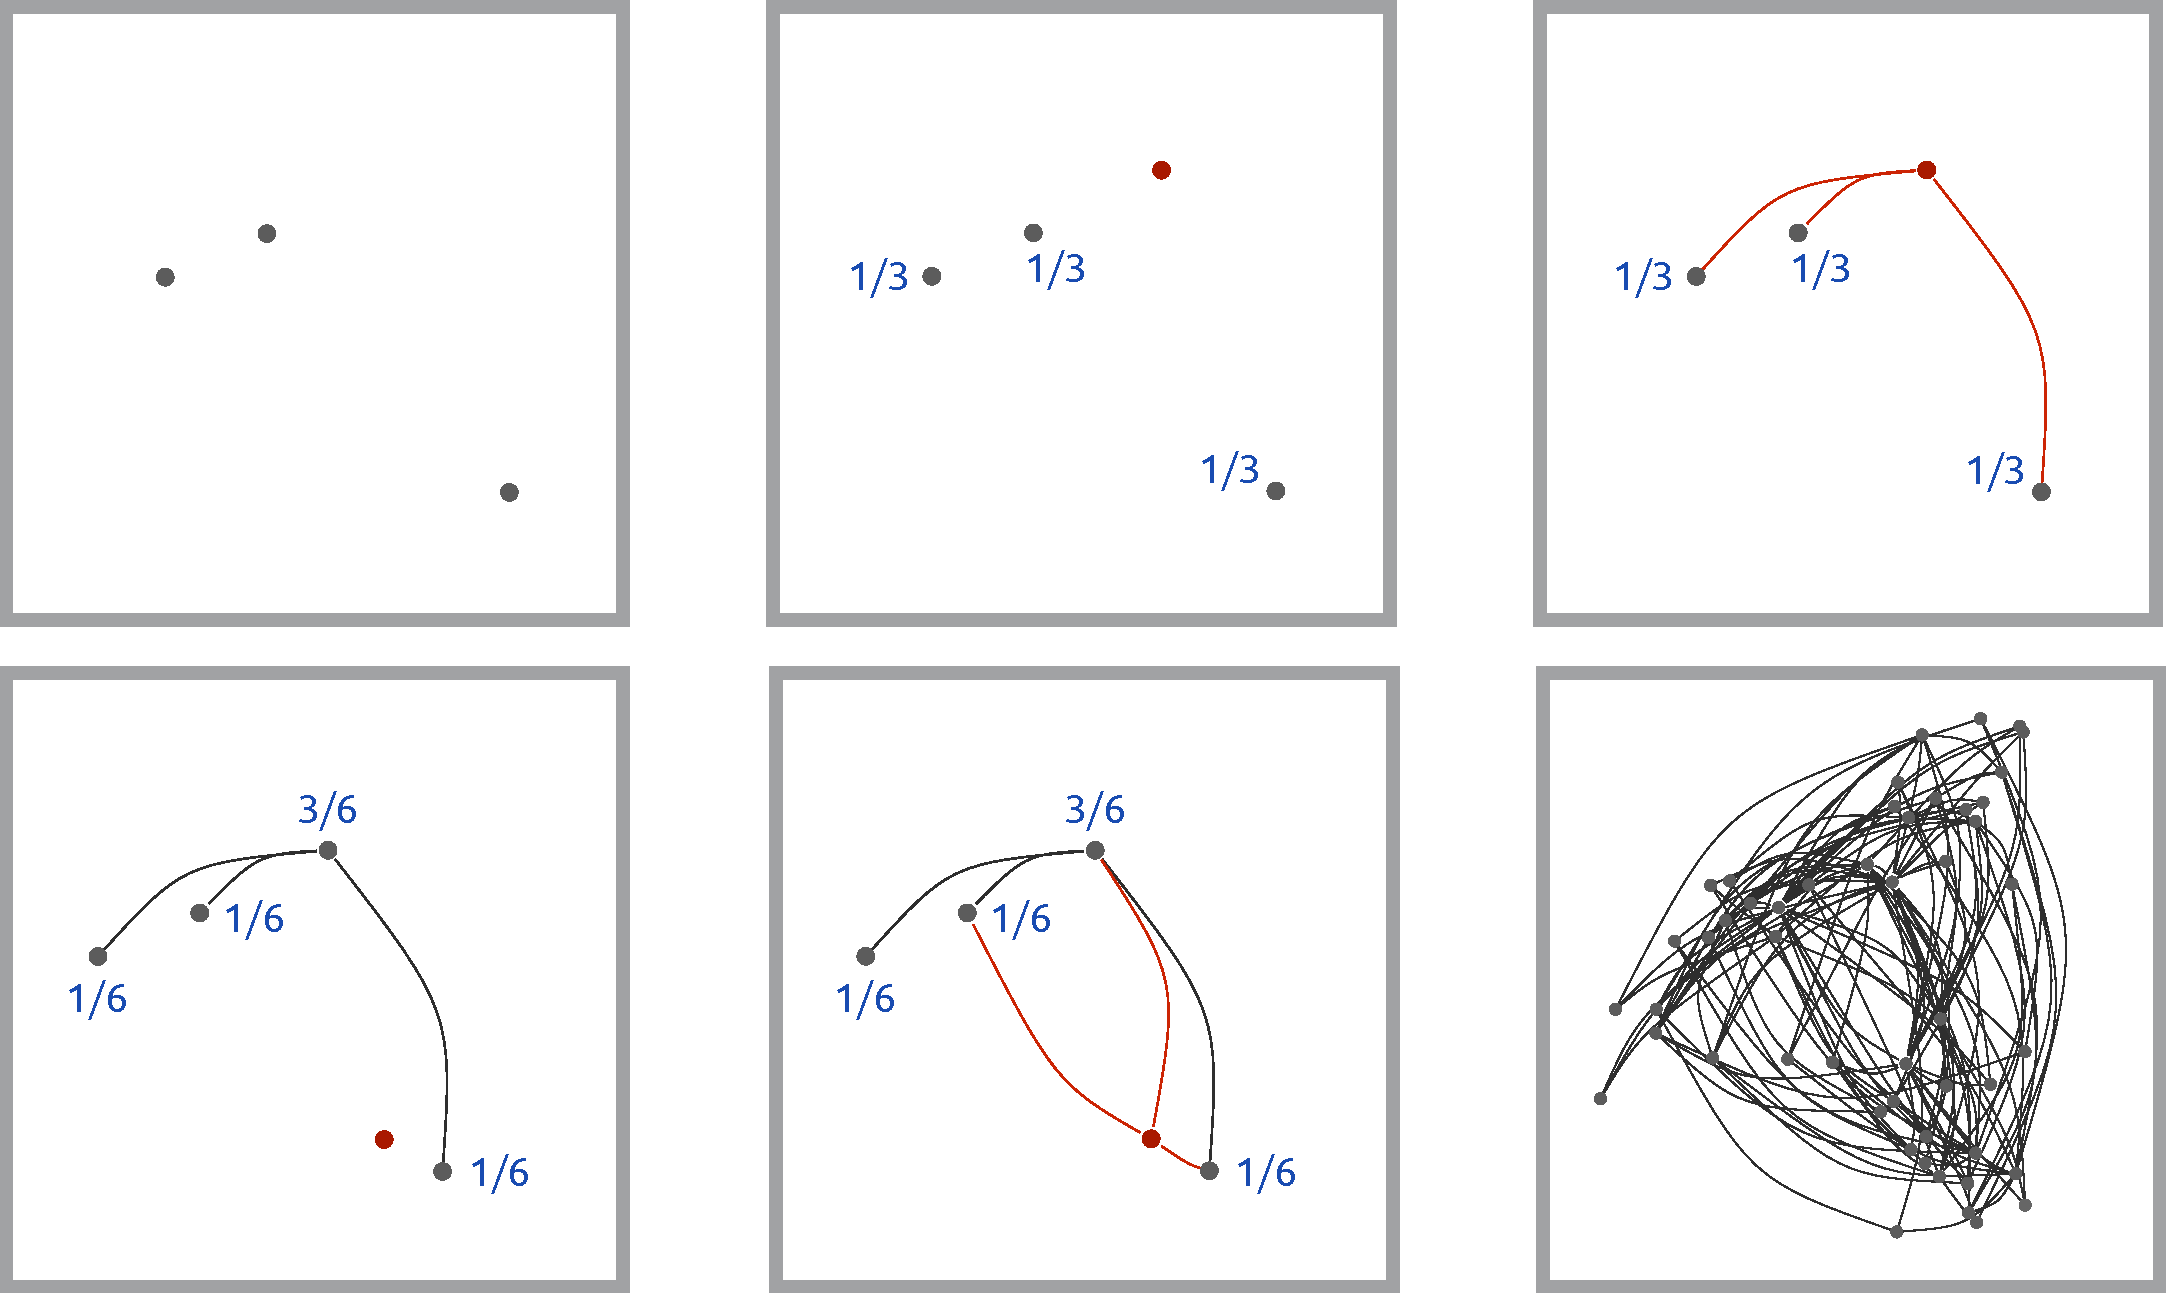
\includegraphics[width=\textwidth]{pictures/21_begin.pdf}
    \caption{The first steps of the Barab\'asi-Albert algorithm with $m
    = m_0 = 3$. From left to right and from top to bottom single nodes are
    first added before edges are chosen according to the preferential
    attachment probabilities printed in blue. The last picture shows the network
    after 47 nodes have been added.}
    \label{fig:21_begin}
\end{figure}

\begin{figure}
    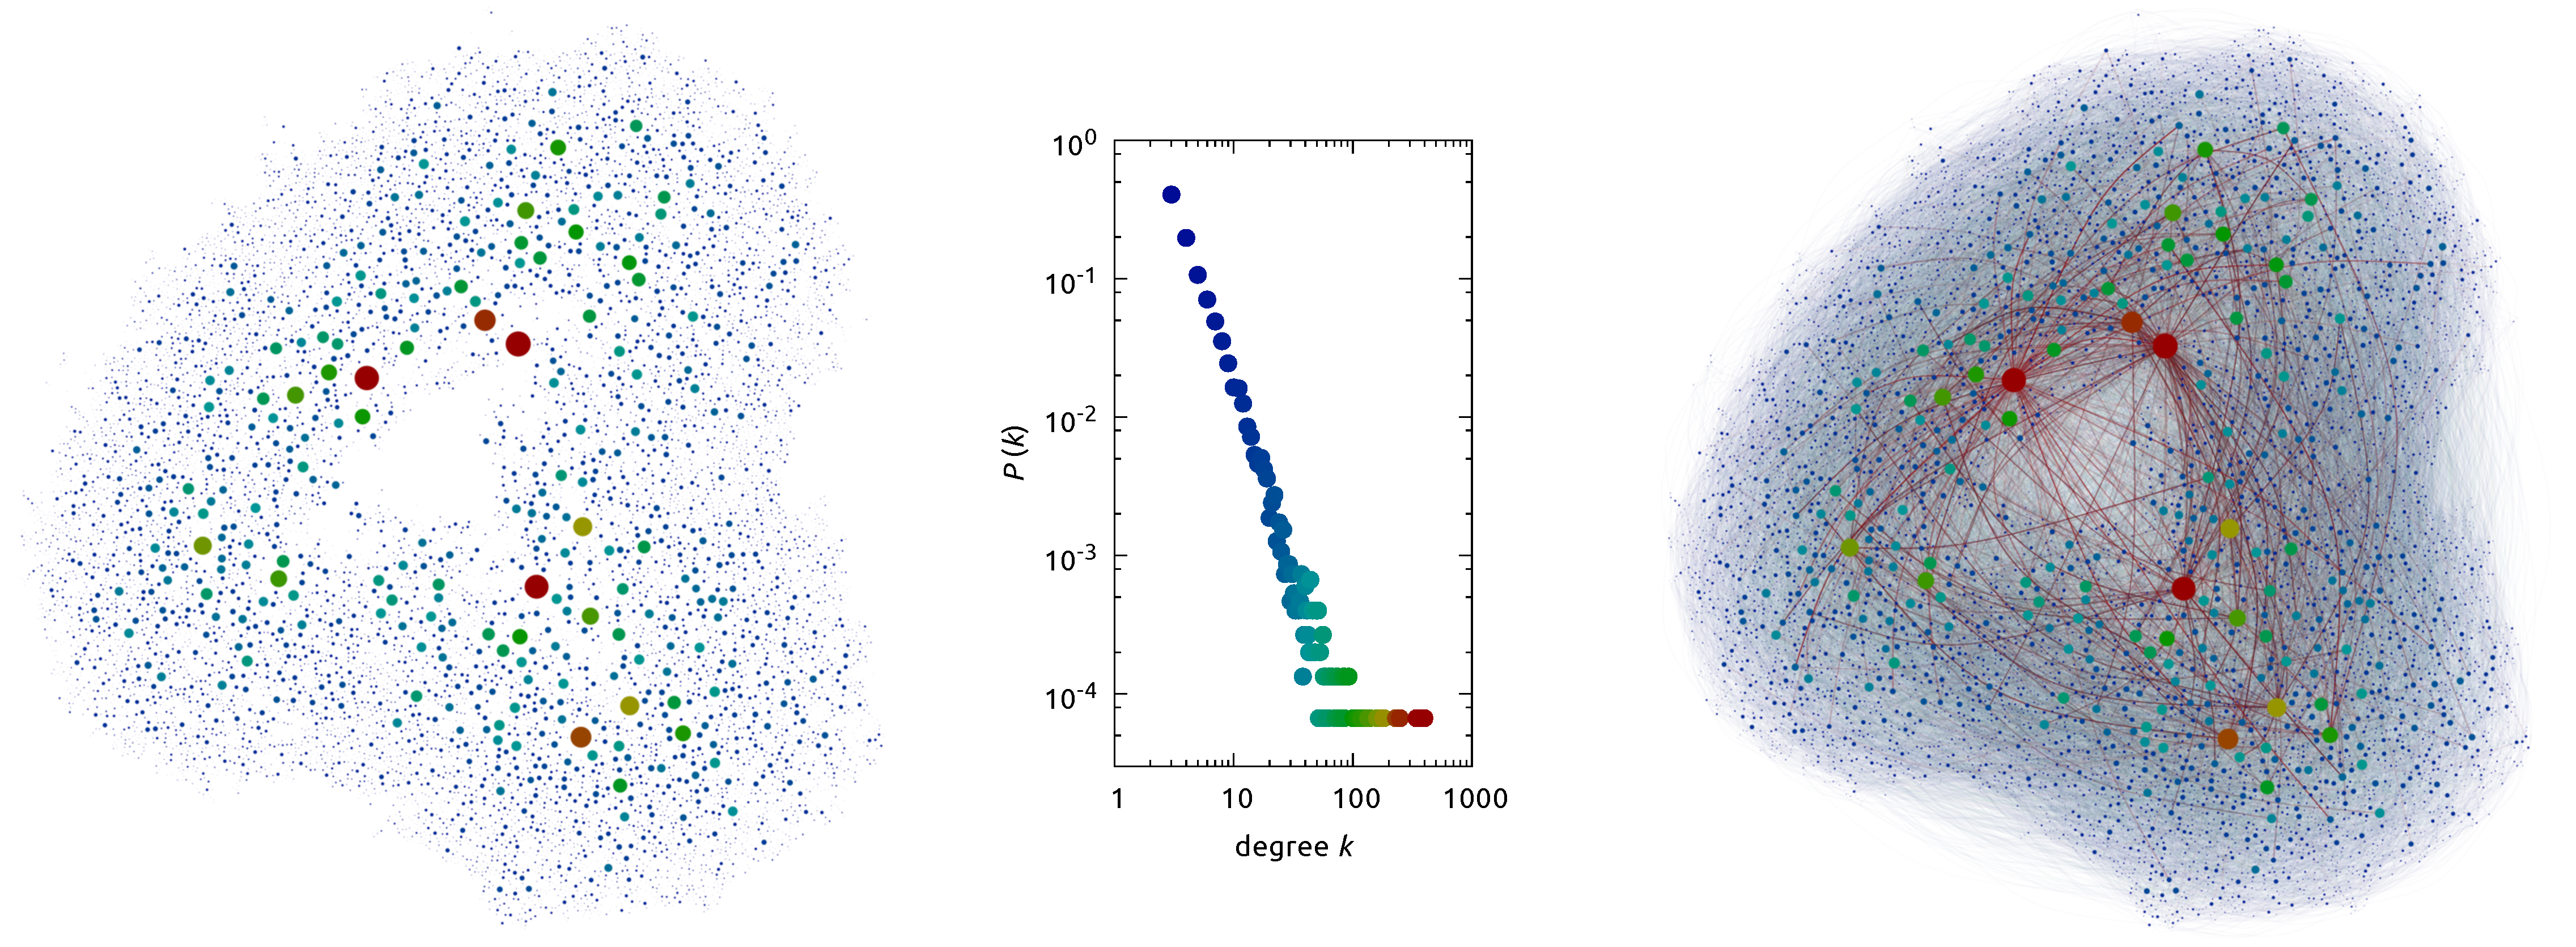
\includegraphics[width=\textwidth]{pictures/21_end.pdf}
    \caption{The same network as in figure \ref{fig:21_begin} after 15000
    nodes have been added (left: without drawing the edges, and right: with
    drawing the edges). The color and the size of the nodes printed in the left
    and right picture describe the degree of the respective node. The
    picture in the middle shows the degree distribution (with the same color
    keys as in the node coloring).}
    \label{fig:21_end}
\end{figure}

\subsection{The Degree Distribution of Barab\'asi-Albert Algorithm}
\begin{figure}
    \gnuplotloadfile[terminal=epslatex, terminaloptions={color size 6,3}]{pictures/22_plot.gp}
    \caption{Degree distribution for a simulation with $N=500000$ nodes
    in total, using different values for $m=m_0$. The line has a slope of
    $-3$.}
    \label{fig:22_plot}
\end{figure}
\begin{figure}
    \gnuplotloadfile[terminal=epslatex, terminaloptions={color size 6,3}]{pictures/22_logplot.gp}
    \caption{The same degree distribution as in figure \ref{fig:22_plot}
    using logarithmic binning so that the the points plotted are the average
    values over equidistant bins on the logarithmic axis (i.e. the bin width
    increases exponentially).}
    \label{fig:22_logplot}
\end{figure}
\clearpage
\section{Random Network Percolation}

\end{document}
